% Especificaciones del tamaño de letra, tamaño de hoja, márgenes, librerias, etc.
\documentclass[12pt, letterpaper]{article}
\usepackage[english]{babel}
\usepackage[utf8]{inputenc}
\usepackage[T1]{fontenc}
\usepackage{amsmath}
\usepackage{graphicx}
\usepackage{subcaption}
\usepackage{hyperref}
\usepackage{url}
\usepackage{amssymb}
\usepackage{float}
\usepackage[margin=1in]{geometry}
\renewcommand{\baselinestretch}{1.5}

% Enlace Bibliografía
\usepackage{csquotes}
\usepackage[notes,backend=biber]{biblatex-chicago}
\addbibresource{referencias.bib}

% Titulo, autores, fecha.
\title{Práctica \#4: Análisis de Flexión}
\author{Carlos Vásquez 1155057}

% Inicio del documento
\begin{document}
\maketitle
\section*{Introducción}
En esta práctica analizaremos las deformaciones que producen las fuerzas que aplicaremos a una barra hueca con un corte en ella. Esto nos permitirá observar las fuerzas que actúan sobre ella y cómo se deforma. Además también podremos observar que cuando aplicamos la fuerza en una arista, es posible obtener una deformación llamada \textit{flexión}, la cual es de interés en nuestros análisis.
\section*{Desarrollo}
La pieza a realizar en CATIA será la siguiente:

\begin{figure}[H]
	\centering
	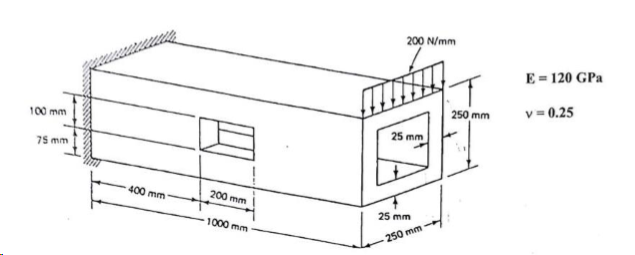
\includegraphics[width=\textwidth]{plane.png}
	\caption{Dimensiones del objeto a modelar.}
\end{figure}

Como podemos observar, la fuerza que se proporcionará a la pieza será de 200 N, pero la dirección de aplicación variará coo veremos a continuación en los anexos de la práctica. Primeramente se analizará la fuerza en una cara de la pieza a compresión, después a tensión y finalmente en la arista, creando la flexión hablada al inicio.

\begin{figure}[H]
	\centering
	\begin{subfigure}[b]{0.7\linewidth}
		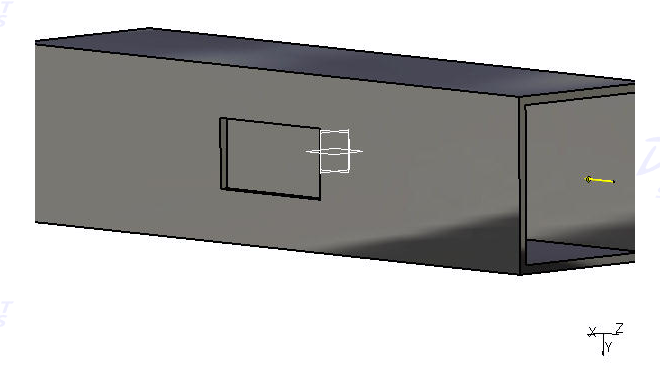
\includegraphics[width=\linewidth]{c1.png}
		\caption{}
	\end{subfigure}
	\begin{subfigure}[b]{0.7\linewidth}
		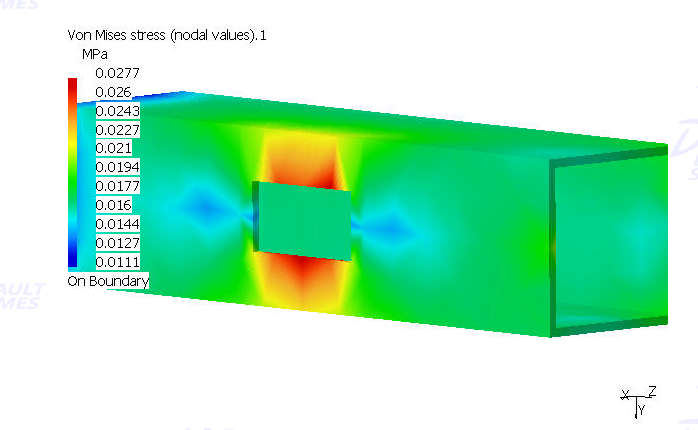
\includegraphics[width=\linewidth]{c2.png}
		\caption{}
	\end{subfigure}
	\caption{Barra a compresión.}
\end{figure}


\begin{figure}[H]
	\centering
	\begin{subfigure}[b]{\linewidth}
		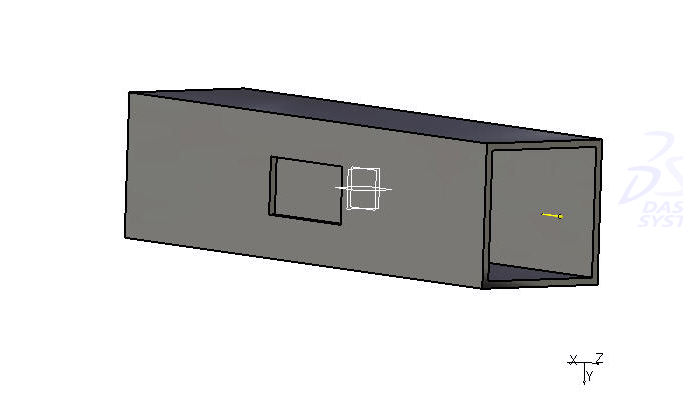
\includegraphics[width=\linewidth]{t1.png}
		\caption{}
	\end{subfigure}
	\begin{subfigure}[b]{\linewidth}
		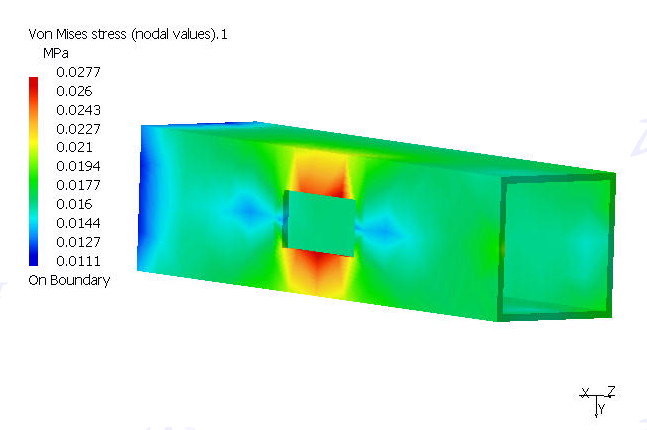
\includegraphics[width=\linewidth]{t2.png}
		\caption{}
	\end{subfigure}
	\caption{Barra a tensión.}
\end{figure}


\begin{figure}[H]
	\centering
	\begin{subfigure}[b]{\linewidth}
		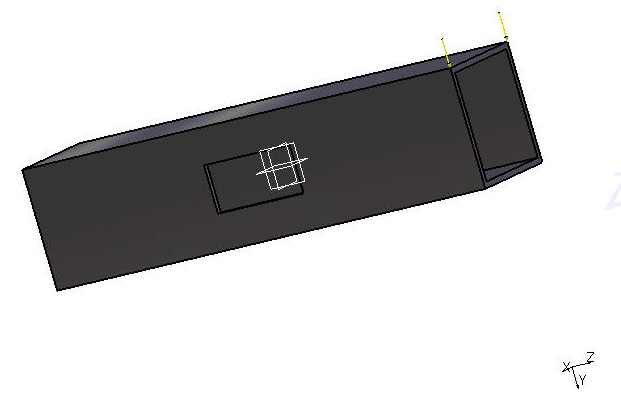
\includegraphics[width=\linewidth]{f1.png}
		\caption{}
	\end{subfigure}
	\begin{subfigure}[b]{\linewidth}
		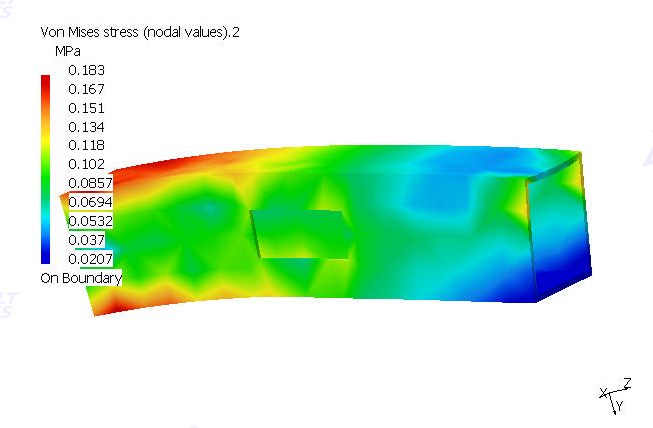
\includegraphics[width=\linewidth]{f2.png}
		\caption{}
	\end{subfigure}
	\caption{Barra con flexión.}
\end{figure}


\section*{Conclusión}
En esta práctica fue sencillo visualizar cómo las fuerzas deforman al cuerpo e incluso los puntos que sufren más estrés gracias a la geometría de la figura. Es de gran ayuda entender y utilizar prorgamas coo CATIA y SOLIDWORKS para realizar estos análisis rápidamente y así comprender las propiedades de los materiales en cuestión, al igual que la geometría más conveniente para éstos.

%%%%%  Bib
\renewcommand\refname{Referencias}
\printbibliography
\end{document}
